\documentclass[10pt, aspectratio=169]{beamer}
\usepackage{tikz}
\usepackage{ngerman}
\usepackage{hyperref}
\usepackage{pdfpages}
\usepackage[most]{tcolorbox}  % 'most' loads libraries like 'listings', 'skins', etc.
\usepackage{xcolor}           % Optional for more color 
\usepackage[dvipsnames]{xcolor}
\usepackage{mathtools}
\beamertemplatenavigationsymbolsempty


\usepackage{style}
\usepackage{graphicx} % Needed for including graphics
\usepackage{caption} % Enhances the caption capabilities
\usepackage{wrapfig}

\setbeamertemplate{footline}
{
  \hbox{\begin{beamercolorbox}[wd=1\paperwidth,ht=2.25ex,dp=1ex,right]{framenumber}%
      \usebeamerfont{framenumber}\insertframenumber{} / \inserttotalframenumber\hspace*{2ex}
    \end{beamercolorbox}}%
  \vskip0pt%
}

% Information to be included in the title page:
\title{\textbf{Komplexität von Code-Problemen}}
\subtitle{Vortrag zum Seminar \\ ``Komplexität''\\\ FG Theoretische Informatik/Formale Methoden}

\author{Ahmad Lowejatan Noori}
\institute{FB Elektrotechnik/Informatik, Universität Kassel}
\date{SoSe 2024}

\begin{document}

\begin{frame}  
    \titlepage
\end{frame}
\begin{frame}{Codes}

\begin{itemize}
    \item Große Rolle in der \alert{Datenübertragungs- bzw. Nachrichtentechnik}
    \item Digitalisierung analoger Signale
    \item Umwandlung von Daten in Bitstrings (Codewörtern)
    \item \alert{Fehlerkorrekturverfahren}
    \item Minimaler Code: höhere Bit-Tiefe $\leftrightsquigarrow$ Überdeckender Code: Abdecken vieler Fehlerzustände
\end{itemize}


\end{frame}

\begin{frame}{Code und Hamming-Ball}


Eine Menge  \textcolor{blue}{$C \subseteq\{0,1\}^n$$, n \in \mathbb{N}$} von \textcolor{blue}{$n$}-stelligen Binärstrings bezeichnen wir als  \alert{Code}.\newline

Def.: \textcolor{blue}{$B_n(u,r)$} ist die Menge aller n-stelligen Binärstrings, die mit höchstens Hamming-Distanz \textcolor{blue}{$r$} von einem zentralen Binärstring \textcolor{blue}{$u$} erreicht werden können. (=\alert{Hamming-Ball} um \textcolor{blue}{$u$})\newline

\end{frame}

%---------------------------------------------------------------%
\begin{frame}{Minimum Radius Problem}
Der \alert{\textbf{Radius}} von Code C,  \textbf{R(C)}, ist das kleinste \textcolor{blue}{$r \in \mathbb{N}$}, sodass gilt: \textcolor{blue}{$C\subseteq B_n(u,r)$} für irgendeinen Binärstring \textcolor{blue}{$u$}.

\begin{columns}[T] % The [T] option aligns the columns' content at the top

    \begin{column}{0.35\textwidth}
        % Your text or content goes here
        \vspace{2em}
        \textbf{\alert{Problem:}}\\
        \textbf{Eingabe:} ein Code  \textcolor{blue}{$C \subseteq \{0,1\}^n$} und \textcolor{blue}{$k \in \mathbb{N}$}\\
        \textbf{Frage:} Ist \textcolor{blue}{$R(C)\leq k$}?
    \end{column}
    \begin{column}{0.4\textwidth}
        \begin{figure}
            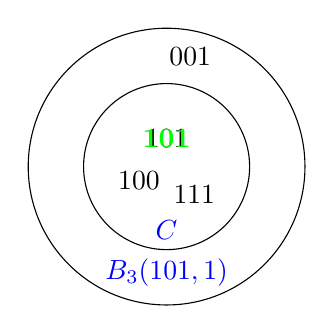
\begin{tikzpicture}
                \draw (0,0) circle (30pt);
                \node<1>[yshift = 1em] {101};
                \node<2->[yshift = 1em] {\textcolor{green}{\textbf{101}}};
                \node[yshift = -1em, xshift = 1em] {111};
                \node[yshift = -0.5em, xshift = -1em] {100};
                \node at (0,-0.8) {\textcolor{blue}{$C$}};
                % The following elements are set to be invisible,
                % if you want them visible remove the opacity setting.
                \draw<2-> (0,0) circle (50pt);
                \node<2-> at (0,-1.35) {\textcolor{blue}{$B_3(101,1)$}};
                \node<2-> at (0.3,1.4) {001};
            \end{tikzpicture}  
            \caption{Beispiel für \textcolor{blue}{$C \subseteq \{0,1\}^3$}, \textcolor{blue}{$B_3(101,1)$}}
            
            \label{fig:example}
        \end{figure}
    \end{column}
\end{columns}
\end{frame}




%--------------------------------------------------%



%--------------------------------------------------%
\begin{frame}{Maximum Covering Radius Problem}
Der \alert{\textbf{Covering Radius}} von Code C,  \textbf{CR(C)}, ist das kleinste \textcolor{blue}{$r\in \mathbb{N} $}, sodass gilt \textcolor{blue}{$\{0,1\}^n =  \bigcup_{u \in C} B_n(u,r)$}
\begin{columns}[T] % The [T] option aligns the columns' content at the top

    \begin{column}{0.35\textwidth}
        % Your text or content goes here
        \vspace{2em}
        \textbf{\alert{Problem:}}\\
        \textbf{Eingabe:} ein Code  \textcolor{blue}{$C \subseteq \{0,1\}^n$ und $k \in \mathbb{N}$}\\
        \textbf{Frage:} Ist \textcolor{blue}{$CR(C)\geq k$}?
        
    \end{column}
    \begin{column}{0.4\textwidth}
     \begin{figure}
    \centering
        \begin{tabular}{|c||c|}
        \hline
            Code C & 2-Ball\\ 
        \hline
             \textbf{101} & \textbf{000}, \textbf{001}, \textbf{011}, \\ &100, 101,\textbf{110} \\ &111 \\ 

        \hline
             \textbf{100} &  000, 001, \textbf{010} \\ &100, 101, 110, \\ & 111 \\ 
        \hline
             \textbf{111} & 001, 010, 011 \\ &100, 101, 110\\ & 111 \\ 
            \hline
        \end{tabular}
    \caption{Beispiel für $C \subseteq \{0,1\}^3$ und alle $v \in B_3(u,2)$ für ein $u\in C$}
    \label{fig:enter-label}
\end{figure}
    \end{column}
\end{columns}

\end{frame}

\begin{frame}{MR und MCR}
\begin{columns}[T] % align columns
\begin{column}{.48\textwidth}

\color{red}\rule{\linewidth}{1pt}

\textbf{Minimum Radius Problem (MR)}\\~\\
\color{black}
\textbf{Eingabe:} ein Code  \textcolor{blue}{$C \subseteq \{0,1\}^n $} und \textcolor{blue}{$k \in \mathbb{N}$}\\
\textbf{Frage:} Ist \textcolor{blue}{$R(C)\le k$}?



\end{column}%
\hfill%

\begin{column}{.48\textwidth}
\color{red}\rule{\linewidth}{1pt}

\textbf{Maximum Covering Radius Problem (MCR)}\\~\\
\color{black}
\textbf{Eingabe:} ein Code  \textcolor{blue}{$C \subseteq \{0,1\}^n$} und \textcolor{blue}{$k \in \mathbb{N}$}\\
\textbf{Frage:} Ist \textcolor{blue}{$CR(C)\geq k$}?
\end{column}%
\end{columns}


\end{frame}




\begin{frame}{Äquivalenz von MR und MCR}
\textbf{Theorem 1}: \textcolor{blue}{ für alle $ C \neq \emptyset,C \subseteq \{0,1\}^n: R(C) + CR(C) = n$ }\\
\textit{Beweisidee über die Form vom CR:}\\
\begin{itemize}
    \item Sei \textcolor{blue}{$r_{max}$} das größte \textcolor{blue}{$r$}, sodass es ein \textcolor{blue}{$v \in \{0,1\}^n$} gibt mit \textcolor{blue}{$B_n(v,r) \cap C = \emptyset$}
    
    \item Mit \textcolor{blue}{$r_{max} + 1$} existiert nun ein Vektor \textcolor{blue}{$u \in C $}, sodass dieser mit höchstens Hamming-Distanz \textcolor{blue}{$r_{max} + 1$} jeden Vektor aus \textcolor{blue}{$\{0,1\}^n \setminus C$} überdeckt, und damit gilt
\end{itemize}
\vspace{2em}
\centering
\textcolor{blue}{
  $\begin{aligned}
        CR(C) &= r_{max}+1 \\ &= \ max\{r \mid \exists v: C \cap B_n(v,r) = \emptyset\}+1
  \end{aligned}$
  }
\end{frame}


\begin{frame}{Äquivalenz von MR und MCR}
\centering{
 \textcolor{blue}{
$\begin{aligned}
  R(C) + CR(C) &= min\{t \mid \exists u: C \subseteq B_n(u,t)\}\ + \\ &\qquad (max\{r \mid \exists v: C \cap B_n(v,r) = \emptyset\}+1)
\end{aligned}$
}
}
\vspace{2em}
\begin{itemize}
    \item Sei \textcolor{blue}{$v \in \{0,1\}^n$}, dann ist \textcolor{blue}{$B_n(v^c,n-r-1)$} das \hyperlink{Kompl}{Komplement} von \textcolor{blue}{$B_n(v,r)$} in \textcolor{blue}{$\{0,1\}^n$}
    
    \item Durch \alert{Bitflipping} hat \textcolor{blue}{ $v^c$} einen Abstand \textcolor{blue}{n} zum Zentrum \textcolor{blue}{$v$}, und erreicht mit höchstens Distanz \textcolor{blue}{$n-r-1$} die restlichen Vektoren des Raums
     \item  Mit \alert{Maximierung} des Hamming-Balls \textcolor{blue}{$B_n(v,r)$} mit \textcolor{blue}{$B_n(v,r)\cap C = \emptyset$}
     , \alert{verkleinert} sich also auch der komplementäre Hamming Ball \textcolor{blue}{$B_n(v^c,n-r-1)$}, wobei \textcolor{blue}{$C \subseteq B_n(v^c,n-r-1)$}
     
\end{itemize}

\vspace{2em}
\textcolor{blue}{
$\begin{aligned}
  \qquad \qquad \qquad &=  \min\{t \mid \exists u: C \subseteq B_n(u,t)\}\ + \\ 
   &\qquad \alert{\max\{r \mid \exists v: C \subseteq B_n(v,n-r-1)\}+1} \\
\end{aligned}$
}
\end{frame}

\begin{frame}{Äquivalenz von MR und MCR}
\centering
\textcolor{blue}{
$\begin{aligned}
  \qquad \qquad \qquad &= \min\{t \mid \exists u: C \subseteq B_n(u,t)\}\ + \\ 
   &\qquad \max\{r \mid \exists v: C \subseteq B_n(v,n-r-1)\}+1 \\~\\
   &\textcolor{black}{\text{Ersetze \textcolor{blue}{$r$} mit \textcolor{blue}{$n-r'-1$}:}}\\
   &= \min\{t \mid \exists u: C \subseteq B_n(u,t)\}\ + 
   \only<1>{\\ & \qquad \alert{\max\{n-r'-1 \mid \exists v: C \subseteq B_n(v,r')\}+1}}
     \only<2>{\\ & \qquad \max\{n-r'-1 \mid \exists v: C \subseteq B_n(v,r')\}+1}\\~\\
    &= \min\{t \mid \exists u: C \subseteq B_n(u,t)\}\ + 
    \only<1>{\\ &\qquad  n-1-\min\{r' \mid \exists v: C \subseteq B_n(v,r')\}+1}
     \only<2>{\\ &\qquad  \alert{n-1-\min\{r' \mid \exists v: C \subseteq B_n(v,r')\}+1}}
    \\~\\
   &= n
\end{aligned}$
}
\end{frame}




\begin{frame}{Äquivalenz von MR und MCR}

\textbf{Beh.:} MR und MCR sind äquivalent\\
\textit{Bew.:}
Aus $R(C)+CR(C)=n$ folgt
\textcolor{blue}{$R(C) \leq k \Leftrightarrow CR(C) \geq n-k$}
\begin{itemize}
    \item MCR und MR aufeinander reduzierbar
    \item Reduktionen offensichtlich polynomiell-zeitbeschränkt
\end{itemize}

$\Rightarrow$ \textbf{Über MR} wird die NP-Vollständigkeit von \textbf{MCR} bewiesen

\end{frame}

\begin{frame}{Eigenschaften von Doppelvektoren}

\textit{Doppelvektoren} sind Vektoren \textcolor{blue}{$v=(v_1v_1v_2v_2\ldots v_nv_n) \in \{0,1\}^{2n}$}
\\~\\

Solche Vektoren haben eine spezielle Eigenschaft, die sich für die spätere Reduktion $3SAT \leq_p MR$ im Zuge der NP-Schwere als nützlich erweisen:\\~\\
\pause
\textbf{Lemma 2:} Für alle \textcolor{blue}{$n > 0$} existiert eine Menge \textcolor{blue}{$Y \subseteq \{0,1\}^{2n}$}, sodass für alle \textcolor{blue}{$v \in \{0,1\}^{2n}$} gilt: \\
\centering{\textcolor{blue}{$v$ ist ein Doppelvektor $\Leftrightarrow$ $Y\subseteq B_{\alert{2n}}(v,\alert{n})$\\}}
\vspace{2em}
\textcolor{blue}{
    $Y := \{(01)^n, (10)^n\} \cup \bigcup_{i=1}^{n} \{(01)^{i-1}10(01)^{n-i}\}
    \cup\bigcup_{i=1}^{n} \{(10)^{i-1}01(10)^{n-i}\}$}
\end{frame}
\begin{frame}{Doppelvektor ist Ball-Zentrum von Y}
\textbf{Lemma 2: }\textcolor{blue}{$v$ ist ein Doppelvektor $\Leftrightarrow$ $Y\subseteq B_{\alert{2n}}(v,\alert{n})$}\\
\textit{Bew.:}\\

$\Rightarrow:$ Sei $v$ ein Doppelvektor. Dann besteht dieser aus einer $n$-fachen Konkatenation von 00- und 11-Blöcken. Die Vektoren aus $Y$ sind gleich lang und bestehen aus 01- oder 10-Blöcken. D.h. Hamming-Distanzen zum Doppelvektor sind \hyperlink{fakt}{\alert{1 für jeden Block}, also \alert{insgesamt $n$.} }\\~\\

$\Leftarrow:$ \textit{Beweisidee:} Über Untermenge von $Y$ zeigen, dass zwei Bits von $v$ gleich sein müssen, dann verallgemeinern\\~\\
Definiere \textcolor{blue}{$Y^i := \{(01)^n, (10)^n,(01)^{i-1}10(01)^{n-i},(10)^{i-1}01(10)^{n-i}\}$}\\~\\
\end{frame}
\begin{frame}{Die ersten zwei Bits sind gleich}
\textit{Beh. 1:} Wenn \textcolor{blue}{$Y^1 \subseteq B_{2n}(v,n)$} für \textcolor{blue}{$v \in \{0,1\}^{2n}$}, dann sind die \alert{ersten zwei Bits gleich.}\\
\textit{Beweisskizze:}
\begin{itemize}
    \item Die maximale Distanz von
    \textcolor{blue}{$v=(v_1v_2\ldots v_{2n}) \in \{0,1\}^{2n}$}
    zu jedem Element aus \textcolor{blue}{$Y^1$} ist höchstens \textcolor{blue}{n} 
    \item max. Distanz setzt sich zusammen  aus:\\
    \textbf{(1)} max. Distanz der ersten \textcolor{blue}{zwei} Bits von \textcolor{blue}{$v \in \{0,1\}^{2n}$} und ein \textcolor{blue}{$y \in Y^1$}\\ \textbf{(2)} max. Distanz der restlichen \textcolor{blue}{$2n-2$} Bits beider Vektoren
 
\end{itemize}
\vspace{1em}
\pause
\begin{columns}[T] % The [T] option aligns the columns' content at the top
    \begin{column}{0.5\textwidth}
     \begin{tabular}{|c||r||l|}
        \hline
           \textcolor{blue}{$Y^{1}$}& Erste \textcolor{blue}{zwei} Bits & Letzte \textcolor{blue}{$2n-2$} Bits \\
        \hline
            \textcolor{blue}{$y_0$} & \textcolor{blue}{01}   & 
            \textcolor{blue}{\only<2>{\colorbox{yellow}{01}0101}\only<3>{01\colorbox{yellow}{01}01}\only<4->{0101\colorbox{yellow}{01}}...01} \\ 
        \hline
           \textcolor{blue}{$y_1$} & 
           \textcolor{blue}{10} &
            \textcolor{blue}{\only<2>{\colorbox{yellow}{10}1010}\only<3>{10\colorbox{yellow}{10}10}\only<4->{1010\colorbox{yellow}{10}}...10} \\
        \hline
            \textcolor{blue}{$y_2$} &
            \textcolor{blue}{01}&
             \textcolor{blue}{\only<2>{\colorbox{yellow}{10}1010}\only<3>{10\colorbox{yellow}{10}10}\only<4->{1010\colorbox{yellow}{10}}...10} \\
        \hline
            \textcolor{blue}{$y_3$}  &
            \textcolor{blue}{10}&
              \textcolor{blue}{\only<2>{\colorbox{yellow}{01}0101}\only<3>{01\colorbox{yellow}{01}01}\only<4->{0101\colorbox{yellow}{01}}...01} \\ 
        \hline
        \end{tabular}
    \end{column}

    \begin{column}{0.5\textwidth}
    \only<5->{
    Offensichtlich gilt für \textbf{(2)} \alert{mindestens} \textcolor{blue}{$n-1$}, da bei jedem \textcolor{blue}{2}-Bit-Block von \textcolor{blue}{$v$} zu einem \textcolor{blue}{2}-Bit-Block von \textcolor{blue}{$y$}  eine \hyperlink{fakt}{Distanz} von \alert{mindestens} 
 \textcolor{blue}{1} entsteht.\\
    D.h. für \textbf{(1)} gilt höchstens \textcolor{blue}{$1$}, und die ersten 2 Bits von \textcolor{blue}{$v$} sind \alert{00} bzw. \alert{11}.
    }
    \end{column}
\end{columns}
\end{frame}
\begin{frame}{Alle Zwei-Bit-Blöcke sind gleich}
\textit{Beh. 2:} Wenn \textcolor{blue}{$Y^i \subseteq B_{2n}(v,n)$} für \textcolor{blue}{$v \in \{0,1\}^{2n}$}, dann ist \textcolor{blue}{$v_{2i} = v_{2i-1}$}\\
\textit{Beweisskizze:} Gilt über Beh. 1 und entsprechender \hyperlink{Versch}{\alert{zirkulärer Bitverschiebung}} nach rechts.\\
\vspace{1em}
Definiere \textcolor{blue}{$Y = Y^1 \cup Y^2 \cup ... \cup Y^n$}. \\Da \textcolor{blue}{$Y^i \subseteq B_{2n}(v,n)$} für alle \textcolor{blue}{i} mit \textcolor{blue}{$1\leq i\leq n$} gilt nach \textit{Beh. 2}, dass \textcolor{blue}{$v$} ein \alert{Doppelvektor} sein muss, wenn \textcolor{blue}{$Y$} im Raum \textcolor{blue}{$\{0,1\}^{2n}$} Teil eines Hamming-Balls mit Radius \textcolor{blue}{$n$} ist.\\
\vspace{1em}
\pause
\textcolor{blue}{$Y$} kann in \textbf{\alert{poly. Zeit}} konstruiert werden, da\\
\vspace{0.3em}
\textcolor{blue}{
    $|Y| = |\{(01)^n, (10)^n\} \cup \bigcup_{i=1}^{n} \{(01)^{i-1}10(01)^{n-i}\}
    \cup\bigcup_{i=1}^{n} \{(10)^{i-1}01(10)^{n-i}\}| = 2n+2$}
\end{frame}
\begin{frame}{MR ist NP-Vollständig}
\textbf{Theorem 2:} Das Minimum Radius Problem ist \alert{NP-Vollständig}\\
\textcolor{blue}{1. MR $\in$ \textbf{NP:}}
\begin{itemize}
    \item Zeuge: \textcolor{blue}{$v \in \{0,1\}^n$} als Zentrum eines Radius-\textcolor{blue}{$k$} Balls, der \textcolor{blue}{$C$} enthält
    \item offensichtlich \alert{polynomiell-längenbeschränkt} in der Größe der Eingabe \textcolor{blue}{$\langle C,k \rangle$}
    \item Verifizierer rechnet und prüft Distanzen zum
    Zeugen durch in \textcolor{blue}{$\mathcal{O}(|C|)$}
    \end{itemize}
\pause
\textcolor{blue}{2. MR ist \textbf{NP}-schwer}\\
Wir zeigen: \alert{3SAT $\leq$ MR}\\
Idee: 
\begin{itemize}
    \item Jede Klausel aus 3CNF \textcolor{blue}{$\varphi$} durch einen Vektor in \textcolor{blue}{$\{0,1\}^{2n}$} repräsentieren 
\item Erfüllende Belegung als \alert{Hamming-Ball-Zentrum}: \textcolor{blue}{Doppelvektor}
    \item Zusammenhänge zwischen Klauselvektoren und Zentrum so kodieren, dass der Code C mit minimalem Radius \textcolor{blue}{$k$} einer erfüllenden Belegung von \textcolor{blue}{$\varphi$} entspricht
\end{itemize}
\end{frame}
\begin{frame}{Kodierung der Klauseln}
Für eine Klausel \textcolor{blue}{$c$} über den Variablen \textcolor{blue}{$x_1,...,x_n$} definieren wie den Vektor \textcolor{blue}{$\hat{c}\in \{0,1\}^{2n}$} folgendermaßen:
\\
für alle \textcolor{blue}{$i = 1,...,n,$} \textcolor{blue}{$\hat{c}_{2i-1}\hat{c}_{2i}=
\begin{cases}
00 & \text{wenn } c \text{ das Literal } \neg x_i \text{ enthält},\\
11 & \text{wenn } c \text{ das Literal } x_i \text{ enthält},\\
01 & \text{sonst}.
\end{cases}$}
\vspace{1em}\\
Definiere \textcolor{blue}{$\Pi: \{0,1\}^n \to \{0,1\}^{2n};$} \textcolor{blue}{$v_1v_2...v_n \mapsto v_1v_1v_2v_2...v_nv_n$}.\\
\vspace{1em}
\textit{Beh. 3:} Sei \textcolor{blue}{$\varphi = c_1 \land ... \land c_t$} eine 3CNF Formel über die Variablen \textcolor{blue}{$x_1,...,x_n$}, dann gilt für beliebige \textcolor{blue}{$v \in \{0,1\}^n$}\\
\begin{center}
    \textcolor{blue}{$\{\hat{c}_1,...,\hat{c}_t\} \subseteq B_{2n}(\Pi(v), n+1)$ }$\Leftrightarrow$ die Belegung \textcolor{blue}{$v$} erfüllt \textcolor{blue}{$\varphi$}
\end{center}
Hierbei wird Belegung \textcolor{blue}{$v$} mit \textcolor{blue}{$\top = 1$} und \textcolor{blue}{$\bot = 0$} kodiert.

\end{frame}
\begin{frame}{Literalblöcke und Belegung}
\pgfsetfillopacity{0.5}
\qquad \textit{Beh. 3:} Sei \textcolor{blue}{$\varphi = c_1 \land ... \land c_t$} eine 3CNF Formel über die Variablen \textcolor{blue}{$x_1,...,x_n$}, dann gilt für\\ \qquad beliebige \textcolor{blue}{$v \in \{0,1\}^n$}\\
\pgfsetfillopacity{0.8}

\begin{center}
   \qquad \textcolor{blue}{$\{\hat{c}_1,...,\hat{c}_t\} \subseteq B_{2n}(\Pi(v), n+1)$ }$\Leftrightarrow$ die Belegung \textcolor{blue}{$v$} erfüllt \textcolor{blue}{$\varphi$}
\end{center}
\pgfsetfillopacity{1}
\noindent
\begin{minipage}[t]{0.5\textwidth}
\textit{Intuition:}
\begin{itemize}
    \item<1-> Jeder Vektor \textcolor{blue}{$\hat{c}$} hat \alert{drei} 11- oder 00-Blöcke und \alert{$n-3$} 01-Blöcke
    \item<2->Hamming-Distanz von \textcolor{blue}{$\Pi(v)$} zu den \textcolor{blue}{$n-3$} 01-Blöcken: \alert{$n-3$}
    \item<3-> Ein Block von \textcolor{blue}{$\Pi(v)$} muss mit \alert{mindestens einem} der drei 11- oder 00-Blöcke übereinstimmen
    \item<4-> Hamming-Distanz von \textcolor{blue}{$\Pi(v)$} zu den drei 11- oder 00-Blöcken: \alert{höchstens $4$}
\end{itemize}
\end{minipage}%
\hspace{1em}
\begin{minipage}[t]{0.4\textwidth}
    Beispiel:\\ \textcolor{blue}{$\varphi' = (\neg x_1 \lor \neg x_2 \lor x_3) \land (x_2 \lor x_4 \lor \neg x_5)$}
           \begin{tabular}{|c||c||c||c||c||c||c|}
        \hline
          \textcolor{blue}{$\varphi'$} & $x_1$ & $x_2$ & $x_3$ & $x_4$ & $x_5$ \\
        \hline
        \textcolor{blue}{$\hat{c}_0$} & \only<1-2>{\textcolor{blue}{00}} \only<3->{\colorbox{yellow}{\textcolor{blue}{00}}} & \textcolor{blue}{00} & \textcolor{blue}{11} & 01 & 01 
             \\
        \hline
           \textcolor{blue}{$\hat{c}_1$} & 01 & \only<1-2>{\textcolor{blue}{11}} \only<3->{\colorbox{yellow}{\textcolor{blue}{11}}} & 01 & \textcolor{blue}{11} & \textcolor{blue}{00}  \\
            \hline
        \alert{$\Pi(v)$} & \only<1-2>{\textcolor{blue}{00}} \only<3->{\colorbox{yellow}{\textcolor{blue}{00}}} &\only<1-2>{\textcolor{blue}{11}} \only<3->{\colorbox{yellow}{\textcolor{blue}{11}}} & \textcolor{blue}{00} & \textcolor{blue}{00} & \textcolor{blue}{11} \\
        \hline
          \textcolor{blue}{$\mathcal{I}(\varphi'$)}& \textcolor{blue}{$\bot$} &\textcolor{blue}{$\top$} & \textcolor{blue}{$\bot$} & \textcolor{blue}{$\bot$} & \textcolor{blue}{$\top$} \\
          \hline
        \end{tabular}
\end{minipage}
\end{frame}
\begin{frame}{Von 3CNF zu Code}

\begin{minipage}[t]{0.5\textwidth}
\begin{itemize}
    \item 3CNF \textcolor{blue}{$\varphi$ = $c_1 \land ... \land c_t$}, Variablen  \textcolor{blue}{$x_1,...,x_n$}
    \item Sei unser konstruiertes \textcolor{blue}{$Y$} nun aus \textcolor{blue}{$\{0,1\}^{2(n+1)}$}
\end{itemize}
Wir definieren Code \textcolor{blue}{$C_\varphi \subseteq \{0,1\}^{2(n+1)}$} wie folgt:
\\
\textcolor{blue}{$C_\varphi = Y \cup \{\hat{c}_100,...,\hat{c}_t00\}$ }
\\

\end{minipage}%    
\begin{tikzpicture}[remember picture, overlay]
\node [anchor=north east, inner sep=0pt, yshift=-5em, xshift=-2em, rounded corners] at (current page.north east) {
    \begin{minipage}[t]{0.5\textwidth}
    \begin{tcolorbox}[colback=blue!5!white,colframe=blue!75!black,title=Erinnerung]
    \small
    \textit{Beh. 3:}
        \textcolor{blue}{$\{\hat{c}_1,...,\hat{c}_t\} \subseteq B_{2n}(\Pi(v), n+1)$ }$\Leftrightarrow$ die Belegung \textcolor{blue}{$v$} erfüllt \textcolor{blue}{$\varphi$}
          \tcblower
    \small
    \textbf{Lemma 2:}
        \textcolor{blue}{$v$ ist ein Doppelvektor $\Leftrightarrow$ $Y\subseteq B_{\alert{2n}}(v,\alert{n})$}
          \end{tcolorbox}
    \end{minipage}
};
\end{tikzpicture}
\\
\textcolor{blue}{$C_\varphi$} ist offensichtlich berechenbar in \alert{\textbf{poly. Zeit}} aus \textcolor{blue}{$\varphi$}.\\
\vspace{1em}
\end{frame}
\begin{frame}{Von 3CNF zu Code}
\begin{center}
    \alert{3SAT $\leq$ MR:} \textcolor{blue}{$\varphi$} ist erfüllbar $\Leftrightarrow$ \textcolor{blue}{$R(C_\varphi) \leq n+1$}
\end{center}

\vspace{1em}
\begin{columns}[T] % The [T] option aligns the columns' content at the top

    \begin{column}{0.5\textwidth}
        % Your text or content goes here
        $\Rightarrow:$\\
        Sei \textcolor{blue}{$\varphi$} erfüllbar. Dann existiert eine erfüllende Belegung \textcolor{blue}{$v \in \{0,1\}^n$}.\\
        \begin{itemize}
            \item Nach \textbf{Lemma 2}: \\\textcolor{blue}{$Y$} \alert{$\subseteq B_{2(n+1)}(\Pi(v)00, n+1)$}
            \item Nach \textit{Beh. 3}: \textcolor{blue}{$\{\hat{c}_1,...,\hat{c}_t\} \subseteq B_{2n}(\Pi(v), n+1)$ }
            \item also auch \textcolor{blue}{$\{\hat{c}_100,...,\hat{c}_t00\}$} \alert{$\subseteq B_{2(n+1)}(\Pi(v)00, n+1)$} 
        \end{itemize}
    \vspace{1em}
    Folglich \textcolor{blue}{$C_\varphi = Y \cup \{\hat{c}_100,...,\hat{c}_t00\} \subseteq  B_{2(n+1)}(\Pi(v)00, n+1) $ }, also \textcolor{blue}{$R(C_\varphi)\leq n+1$}
    \end{column}
    \begin{column}{0.5\textwidth}
        $\Leftarrow:$\\
        Sei \textcolor{blue}{$b \in \{0,1\}^{2(n+1)}$} Zentrum eines Balls mit Radius \textcolor{blue}{$n+1$}, in dem \textcolor{blue}{$C_\varphi$} enthalten ist.
        \begin{itemize}
            \item \textcolor{blue}{$Y$} \alert{$\subseteq B_{2(n+1)}(b,n+1)$}
            \item Nach\textbf{ Lemma 2}: \\ \textcolor{blue}{$b$} ist also Doppelvektor
            \item Sei \textcolor{blue}{$b' \in \{0,1\}^{2n}$} wie \textcolor{blue}{$b$} ohne den letzten 00/11-Block, dann existiert \textcolor{blue}{$v \in \{0,1\}^n$} mit \textcolor{blue}{$\Pi(v) = b'$}
            \item \textcolor{blue}{$\{\hat{c}_100,...,\hat{c}_t00\} \subseteq B_{2(n+1)}(b, n+1)$ } 
            \item also auch  \textcolor{blue}{$\{\hat{c}_1,...,\hat{c}_t\}$} \alert{$\subseteq B_{2n}(\Pi(v), n+1)$ }
        \end{itemize}
        \vspace{0.4em}

    Folglich ist \textcolor{blue}{$v$} nach \textit{Beh. 3} eine erfüllende Belegung und damit \textcolor{blue}{$\varphi$} erfüllbar.
    \end{column}
    
\end{columns}
\end{frame}
\begin{frame}{MCR ist NP-Vollständig}
\textit{Beh.:} Das \textbf{Maximum Covering Radius Problem} ist NP-Vollständig\\

\textit{Bew.:} folgt sofort aus \alert{\textbf{Äquivalenz}} von \textbf{MCR und MR} und \alert{\textbf{NP-Vollständigkeit}} von \textbf{MR}
\end{frame}
\begin{frame}{Ausblick}
\begin{minipage}[t]{0.5\textwidth}
    \begin{itemize}
    \item Weiteres Anwendungsgebiet: \hyperlink{Ham}{\alert{Consensussequenz}} in der Genetik
    \item Def.: Funktionell wichtige DNA- oder Proteinsequenz, die bei verschiedenen Organismen weitgehend übereinstimmt, aber \alert{nicht} identisch ist 
    \item Viele ``effiziente'' Algorithmen sind metaheuristisch
    
\end{itemize}
\end{minipage}%


\begin{tikzpicture}[remember picture, overlay]
\node [anchor=north east, inner sep=0pt, yshift=-8
em, xshift=-2em, rounded corners] at (current page.north east) {
    \begin{minipage}[t]{0.5\textwidth}
    \begin{tcolorbox}[colback=blue!5!white,colframe=blue!75!black,title=Beispiele für Metaheuristiken]
    \small
    \begin{itemize}
        \item[1.] Bestimme eine Startlösung L
        \item[2.] Definiere eine \textit{Nachbarschaft} von zu L ``ähnlichen'' Lösungen 
        \item[3.] Suche diese Nachbarschaft vollständig ab und bestimme die beste Lösung 
    \end{itemize}
        
          \end{tcolorbox}
    \end{minipage}
};
\end{tikzpicture}
\end{frame}

\begin{frame}{Literatur}
\begin{thebibliography}{9}

\bibitem{1} Frances, M., Litman, A. On covering problems of codes. Theory of Computing Systems 30, 113–119 (1997). https://doi.org/10.1007/BF02679443
\bibitem{2} Festa, P., Pardalos, P.M. Efficient solutions for the far from most string problem. Ann Oper Res 196, 663–682 (2012). https://doi.org/10.1007/s10479-011-1028-7

\end{thebibliography}


\end{frame}
\setbeamertemplate{footline}{}

\begin{frame}[label = {Ham}]{Hamming-Distanz}
\addtocounter{framenumber}{-1}
\begin{itemize}
    \item Codes sind nicht nur auf binärem Alphabet beschränkt
    \item \textcolor{blue}{$\Sigma=\{c_1,c_2,...,c_k\}, u,v \in \Sigma^m$}
    \item \textcolor{blue}{$d(u,v)=\sum_{i=1}^m\Phi(u_i,v_i)$}
    \item \textcolor{blue}{$\Phi: \Sigma \times \Sigma \rightarrow \{0,1\}, \Phi(a,b) =
    \begin{cases}
0 & \text{wenn } a = b,\\
1 & \text{sonst}.
\end{cases}$}
\end{itemize}
\end{frame}

\begin{frame}[label={fakt}]{Fakten über Hamming-Distanzen}
\addtocounter{framenumber}{-1}

\begin{enumerate}
    \item Seien \textcolor{blue}{$u_1, u_2$} und \textcolor{blue}{$v_1, v_2$} Binärstrings mit \textcolor{blue}{$|u_1| = |u_2|$} und \textcolor{blue}{$|v_1| = |v_2|$}, dann gilt 
   \textcolor{blue}{ $d(u_1v_1, u_2v_2) = d(u_1,u_2) + d(v_1, v_2)$}

   \item {Für beliebige \textcolor{blue}{$u,v\in\{0,1\}^n: d(u,v) + d(u^c,v) = n$}}
   
\end{enumerate}
\end{frame}
\begin{frame}[label ={Kompl}]{Hamming-Ball Komplement}
\addtocounter{framenumber}{-1}
\textit{Beh.: }Sei \textcolor{blue}{$v \in \{0,1\}^n$}, dann ist \textcolor{blue}{$B_n(v^c,n-r-1)$} das Komplement von \textcolor{blue}{$B_n(v,r)$} in \textcolor{blue}{$\{0,1\}^n$}\\

\textit{Bew.: }\textcolor{blue}{
\begin{align}
v \not \in B_n(v,r) &\Leftrightarrow d(u,v) > r\\
 &\Leftrightarrow d(u^c,v) < n-r\\
  &\Leftrightarrow v \in B_n(u^c, n-r-1)
\end{align}}

\textcolor{blue}{(2)} folgt aus \textcolor{blue}{$d(u,v)+d(u^c,v) = n$}
\end{frame}

\begin{frame}[label = {Versch}]{Zirkuläre Rechtsverschiebung}
\addtocounter{framenumber}{-1}
\begin{tikzpicture}[remember picture, overlay]
\node [anchor=north east, inner sep=0pt, yshift=-5em, xshift=-2em, rounded corners] at (current page.north east) {
\begin{minipage}[t]{0.3\textwidth}
    \begin{tcolorbox}[colback=blue!5!white,colframe=blue!75!black,title=Beispiel: \\2-Bit-Verschiebung]
        \begin{tabular}{c|c|c|c|c}
        \hline
          1 & 0 & 1 & \textcolor{blue}{1} & \textcolor{blue}{0}\\
         \hline
        \end{tabular}\\
        \begin{tabular}{c|c|c|c|c}
        \hline
          \textcolor{blue}{0} & 1 & 0 & 1 & \textcolor{blue}{1}\\
         \hline
        \end{tabular}\\
        \begin{tabular}{c|c|c|c|c}
        \hline
          \textcolor{blue}{1} &   \textcolor{blue}{0} & 1 & 0 & 1\\
         \hline
        \end{tabular}
    \end{tcolorbox}
      \begin{tcolorbox}[colback=blue!5!white,colframe=blue!75!black,title=Erinnerung]
       \textcolor{blue}{$Y^i = \{(01)^n, (10)^n,\\(01)^{i-1}10(01)^{n-i},\\(10)^{i-1}01(10)^{n-i}\}$}
    \end{tcolorbox}
\end{minipage}
};
\end{tikzpicture}

\begin{minipage}[t]{0.7\textwidth}
    Sei \textcolor{blue}{$S_i: \{0,1\}^{2n} \rightarrow \{0,1\}^{2n}$} die zirkuläre Rechtsverschiebung eines Vektors um \textcolor{blue}{$2i-2$} Bits.
    Für \textcolor{blue}{$i=1,...,n$} definieren wir\\
    \textcolor{blue}{$Y^i = S_i(Y^1)$}.\vspace{1em}\\
    \textit{Beh. 2:} Wenn \textcolor{blue}{$Y^i \subseteq B_{2n}(v,n)$} für \textcolor{blue}{$v \in \{0,1\}^{2n}$}, dann ist \textcolor{blue}{$v_{2i} = v_{2i-1}$}\\
\textit{Bew.:}
\begin{itemize}
    \item \textcolor{blue}{$S_i$} ist ein Isomorphismus, also auch eine bijektive (distanzen-erhaltende) Abbildung
    \item Folglich gilt für alle \textcolor{blue}{$i$}:\\ \textcolor{blue}{$Y^i \subseteq B_{2n}(v,n) \Leftrightarrow Y^1 \subseteq B_{2n}(S_i^{-1}(v),n)$}
    \item Es gilt also auch für beliebige \textcolor{blue}{$v \in \{0,1\}^{2n}: v_{2i-1}=v_{2i} \Leftrightarrow (S_i^{-1}(v))_1 = (S_i^{-1}(v))_2$}. (nach Beh. 1)
\end{itemize}

\end{minipage}
\end{frame}
\end{document}
